\section{Creating a behavior tree structure}
    There are several possible approaches to creating a BT structure. We will present a few of these approaches and state the used one. In this section, we used the insight from \cite{BT_creation}.\\
    The first approach is creating the complete BT by hand. Meaning that humans must design every node and its position and function within the structure.\\
    The second approach is creating an initial BT and letting RL algorithms improve their functionality and optimality. There are several options for this particular approach.\\
    The third possible approach is constructing the BT from previously recorded human behavior.\\
    The last possible approach lets the RL algorithm construct the BT structure from scratch.\\
    Each of the presented approaches has its advantages and disadvantages. It is, therefore, vital to select the correct approach based on the possibilities and requirements of the task.\\\\
    \bfc{Chosen approach}\\
        We have chosen the first approach, meaning we will construct the whole tree structure by hand. This was done as it is the easiest approach to this task and requires no additional steps.\\
        Using different approaches to designing and improving the BT structure may be an interesting task for future work.\\
        We will design the BT structure in the GUI application designed alongside our chosen BT library, Groot. The application interface is shown in figure \ref{fig:groot}.\\\\
        \begin{figure}[ht]
            \centering
            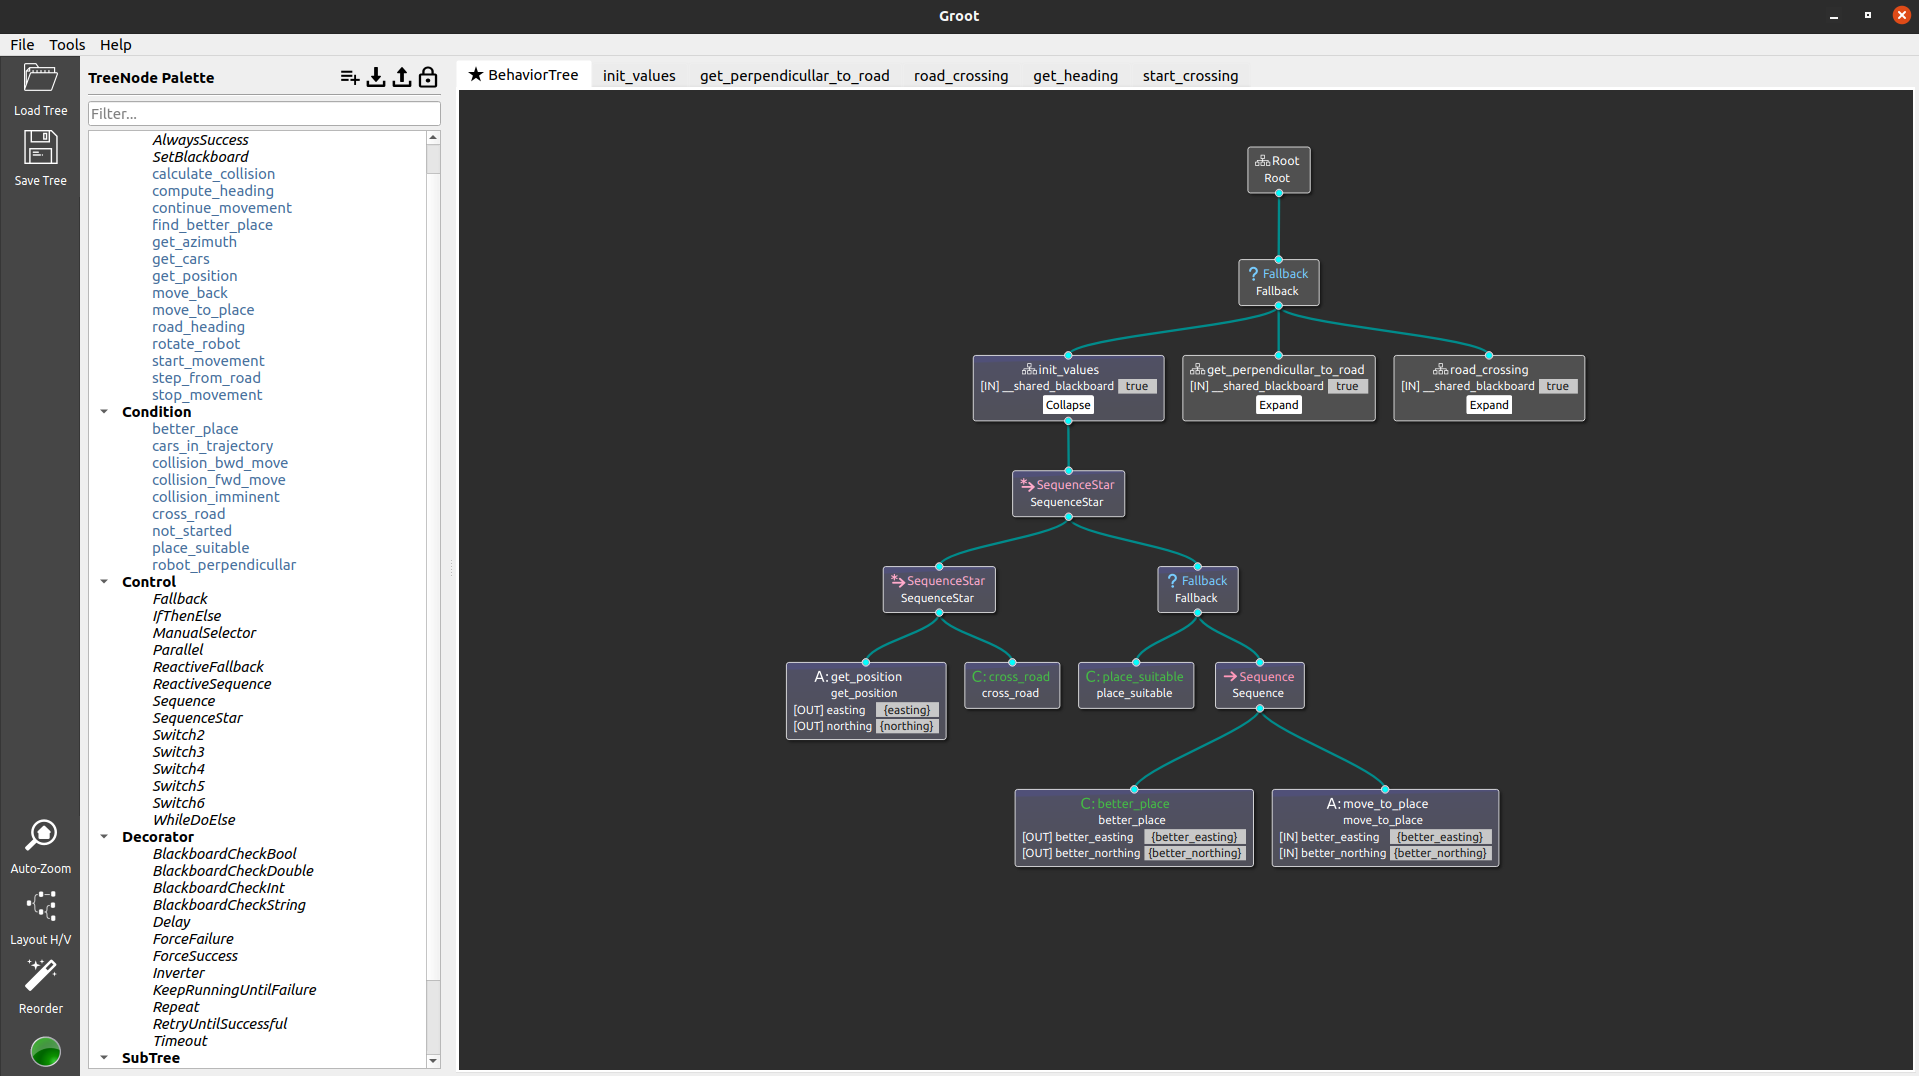
\includegraphics[width=\linewidth]{images/Groot.png}
            \caption{The Groot application interface.}
            \label{fig:groot}
        \end{figure}
    

\section{Structure hierarchy -- Main BT}
    We will divide the whole tree structure into several sub-trees to help with readability, modularity, and maintainability.\\
    The first sub-tree will help with initialization and will be responsible for determining whether the tree should be run. It is also responsible for navigating the robot to a suitable crossing place. This sub-tree will be called \texttt{Init-BT}.\\
    The second sub-tree will be responsible for positioning the robot such that it is perpendicular to the road it is trying to cross. This sub-tree will be called \texttt{Perpendicular-BT}.\\
    The third sub-tree will be responsible for the navigation of the robot during the crossing. It will check the positions and speed of incoming traffic and determine the best strategy for the crossing. This sub-tree will be called \texttt{Crossing-BT}.\\
    There are a few more sub-trees in our structure, but those are not that important to write about here. They will be presented when they are mentioned in the main sub-trees structure. Their main task is to help with the modularity and reusability of the behavior they encode.\\
    The main BT is shown in figure \ref{fig:main-BT}.\\
    \begin{figure}[ht]
        \begin{tikzpicture}[sibling distance=30mm, minimum width=1cm, minimum height=0.8cm]
            \node [draw] {$Root$}
                child {node [draw] {$\to$} edge from parent [-{Stealth[length=2.5mm]}]
                child {node [ellipse, draw] {StartAlgorithm}}
                child {node [draw] {$\to^{*}$}
                child {node [draw] {$\to^{*}$}
                child {node [diamond, draw, aspect=2.3, xshift=0-0.4cm, yshift=0-0.5cm] {Init}}
                child {node [diamond, draw, aspect=2.9, yshift=0-0.5cm] {Perpendicular}}}
                child {node [diamond, draw, aspect=2.3] {Crossing}}}};
        \end{tikzpicture}
        \caption{Main BT structure.}
        \label{fig:main-BT}
    \end{figure}
    The main BT starts with a \texttt{Sequence} node. First, we need to check if the algorithm should be even started -- to avoid collision between two nodes trying to control the robot. This we achieve with a condition node \texttt{StartAlgorithm} node. This node will check if the algorithm should be started. If it should not, the algorithm will not progress. The second child is a \texttt{SequenceStar} node. This node will tick the sub-trees responsible for the whole algorithm.\\
    However, the first child is a \texttt{SequenceStar} node. This is done to ensure that each of the preparation sub-trees will be executed once (that is, if they return \texttt{SUCCESS}).\\
    The first preparation sub-tree is the \texttt{Init-BT}, its structure shown in chapter \ref{sec:Init-BT} and its implementation in chapter \ref{sec:Init-BT-impl}.\\
    The second preparation sub-tree is the \texttt{Perpendicular-BT}, its structure shown in chapter \ref{sec:Perpendicular-BT} and its implementation in chapter \ref{sec:Perpendicular-BT-impl}.\\
    The last sub-tree is the \texttt{Crossing-BT}, its structure shown in chapter \ref{sec:Crossing-BT} and its implementation in chapter \ref{sec:Crossing-BT-impl}.

\section{Init BT}
\label{sec:Init-BT}
    As mentioned earlier, this BT is responsible for determining if we should start the crossing and for navigating the robot to the optimal location. This tree will be executed only once for each crossing. We accomplish this with a \texttt{SequenceStar} node as the first node after \texttt{Root}. The \texttt{Init-BT} structure is shown in figure \ref{fig:Init-BT}.\\
    \begin{figure}[ht]
        \begin{tikzpicture}[sibling distance=28mm, minimum width=1cm, minimum height=0.8cm]
            \node [draw] {$Root$}
                child {node [draw] {$\to$} edge from parent [-{Stealth[length=2.5mm]}]
                child {node [draw, xshift=0-1.6cm] {$\to^{*}$}
                child {node [draw] {GetPosition}}
                child {node [ellipse, draw] {CrossRoad}}}
                child {node [draw, xshift=1.6cm] {?}
                child {node [ellipse, draw, xshift=0.2cm] {PlaceSuitable}}
                child {node [draw] {?}
                child {node [draw] {$\to$}
                child {node [ellipse, draw, xshift=0-0.1cm] {BetterPlace}}
                child {node [draw, xshift=0.1cm] {MoveToPlace}}}
                child {node [draw, xshift=0-0.2cm] {GetBetterPlace}}
                child {node [ellipse, draw, xshift=0-0.6cm] {$\checkmark$}}}}};
        \end{tikzpicture}
        \caption{The Init-BT structure.}
        \label{fig:Init-BT}
    \end{figure}
    The flow for the algorithm is the following. We start at a \texttt{Sequence} node. With its first child being a control node \texttt{SequenceStar}, we start the \texttt{Init-BTs} first branch. The first node in this branch is an action node \texttt{GetPosition} followed by a condition node \texttt{CrossRoad}. The idea behind this branch is to determine the proximity of the robot to the road. If the robot is too far away from the road, the algorithm should not progress. This will help combat the possibility of trying to cross the wrong road, should it happen that two roads are close by.\\
    The second branch of this sub-tree starts with a \texttt{Fallback} node. The idea behind this branch is to place the robot in an ideal position for crossing. This action should have been done before the mission, and the robot should have been sent to the optimal location by a path-planning node.\\
    However, if such pre-mission planning was not performed, the \texttt{PlaceSuitable} condition node will check if the place is suitable. If not, the \texttt{BetterPlace} condition node will return if a better location was found. An action node \texttt{MoveToPlace} will steer the robot to a better location if it has been found. Lastly, the action node \texttt{GetBetterPlace} will try to find a better place.\\
    We will not perform the sub-tree again if a better place cannot be located. Instead, we will move on to the following sub-tree and cross the road in the position the robot is currently situated. This is done to avoid an infinite loop and is achieved with a \texttt{ReturnSuccess} node at the end of the second branch.\\

\section{Perpendicular BT}
\label{sec:Perpendicular-BT}
    This sub-tree is responsible for positioning the robot for crossing in the most optimal way. We have determined that to be the one in which the robot will cross the road the fastest. As such, the position of the robot should be perpendicular to the road it is going to cross. Figure \ref{fig:Perpendicular-BT} shows the BT structure for achieving so.\\
    \begin{figure}[ht]
        \begin{tikzpicture}[sibling distance=28mm, minimum width=1cm, minimum height=0.8cm]
            \node [draw] {$Root$}
                child {node [draw] {$\to^{*}$} edge from parent [-{Stealth[length=2.5mm]}]
                child {node [draw] {$\to^{*}$}
                child {node [draw] {$\circ(10)$}
                child {node [draw] {GetAzimuth}}}
                child {node [draw, xshift=0-0.7cm] {$\circ(10)$}
                child {node [draw] {$\to$}
                child {node [draw, xshift=0.65cm] {GetPosition}}
                child {node [draw, xshift=0.35cm] {RoadHeading}}
                child {node [draw, xshift=0.5cm] {ComputeHeading}}}}}
                child {node [draw, xshift=3cm] {$\circ(10)$}
                child {node [draw] {$\to$}
                child {node [draw] {GetAzimuth}}
                child {node [draw] {?}
                child {node [ellipse, draw, xshift=0-0.5cm, yshift=0-1.5cm] {RobotPerpendicular}}
                child {node [draw] {$\times$}
                child {node [draw] {?}
                child {node [draw, xshift=0-1.2cm] {RotateRobot}}
                child {node [draw, xshift=0-1.2cm] {StepFromRoad}}}}}}}};
        \end{tikzpicture}
        \caption{The Perpendicular-BT structure.}
        \label{fig:Perpendicular-BT}
    \end{figure}
    The first branch of this tree is also only needed once in each run of the crossing algorithm. Therefore, the first node after the \texttt{Root} node is a \texttt{SequenceStar} control node.\\
    The task of the first branch is to determine the azimuth for the robot to be perpendicular to the road. This also does not need to be repeated for a single road, so we start with a \texttt{SequenceStar} node, next, we have a \texttt{Repeat} node. The action to be repeated is the obtaining of the robot's azimuth. The following steps are also behind a \texttt{Repeat} control node. This part of the algorithm calculates the azimuth the robot should have to be perpendicular. Firstly we need to obtain the robot's position -- \texttt{GetPosition} action node. Next, we need to determine the road heading closest to the robot. For this purpose, we have the action node \texttt{RoadHeading}. Finally, we calculate the proper azimuth for the robot with the action node \texttt{ComputeHeading}. This concludes the left branch of our Perpendicular-BT.\\
    The right branch starts with a \texttt{Repeat} node, followed by a \texttt{Sequence} node. The idea behind this branch is to utilize the azimuth value computed in the left branch and orient the robot accordingly. Firstly we need to obtain the robot's azimuth with the \texttt{GetAzimuth} action node. While this might seem redundant, we have just got the azimuth for calculation, it is vital to update the current azimuth as the value of obtained azimuth is only valid in the first run of the second branch. After receiving the current azimuth, we follow with a \texttt{Fallback} node and its first child, a condition node \texttt{RobotPerpendicular}. This node tells us if the robot has achieved the optimal azimuth we calculated earlier. If it has not, we continue, thanks to the \texttt{Fallback} node to the last part of this sub-tree. We want this part to always return \texttt{FAILURE}. This is necessary because we check the correct position before the movement. The last part is responsible for the movement of the robot. Firstly we try to rotate the robot with \texttt{RotateRobot} action node. If the rotation was unsuccessful, we tried to move the robot away from the road with \texttt{StepFromRoad}. This is implemented as the robot rotation could have brought the robot onto the road, which is forbidden.\\
    While we could unite the first two \texttt{Repeat} nodes, maybe even all three, we chose not to do so. The reason for not merging the nodes is to allow each algorithm part to fail independently. The number of repetitions for each node was set to 10, which we determined to be the optimal value.

\section{Crossing BT}
\label{sec:Crossing-BT}
    This tree is the most important part of the whole algorithm as it facilitates road crossing. Figure \ref{fig:Crossing-BT} shows the structure of the tree.\\
    This tree starts in the \texttt{Sequence} node with five children. This tree also contains two further sub-trees. These sub-trees are shown in figures \ref{fig:StartMovement-BT} and \ref{fig:Finished-BT}, and will be explained separately at the end of this section.\\
    The first branch of this tree is responsible for obtaining the data of all detected vehicles from other ROS nodes. This functionality is implemented in just one action node \texttt{GetCars}.\\
    The second branch starts with the \texttt{Fallback} node. The first child of this node is a condition node \texttt{CarsInTrajectory}. This node checks if any cars are in the robot's trajectory. If there are not, we are free to continue with our movement or start it if we have not done so yet. This is performed with a sub-tree \texttt{StartCrossing}, followed by the \texttt{ContinueMovement} action node. These nodes are connected behind a \texttt{Sequence} node.\\
    The following two branches are responsible for crossing the road if cars are detected in the robot's trajectory. The third node is the \texttt{StartCrossing} sub-tree.\\
    The fourth branch is the decision-making part of the tree. It starts with the \texttt{Sequence} node with its first child, the \texttt{CalculateCollision} action node. This node is responsible for calculating the velocities for the robot to collide with all detected vehicles. These velocities are vital information on which all the decision-making is based.\\
    The second child of the \texttt{Sequence} node is a structure of cascading if-else statements. The structure gradually checks the following conditions and performs the corresponding actions based on the results.\\
    The first condition is the \texttt{CollisionImminent} condition node. This node checks if the robot is about to collide with any of the detected vehicles. If it is not, the robot will continue its current movement.\\
    If a collision is detected, we check if the collision would be on moving forward with a \texttt{CollisionFwdMove}. If not, we can continue with the forward movement. However, the speed could change.\\
    If the collision would be on forward movement, we check if the robot can move backward with a \texttt{CollisionBwdMove} condition node. If it can, we move backward with the \texttt{MoveBwd} node. If not, we stop the robot using the \texttt{StopMovement}.\\
    \begin{figure}[H]
        \begin{tikzpicture}[sibling distance=28mm, minimum width=1cm, minimum height=0.8cm]
            \node [draw] {$Root$}
                child {node [draw] {$\to$} edge from parent [-{Stealth[length=2.5mm]}]
                child {node [draw] {GetCars}}
                child {node [draw] {?}
                child {node [draw, xshift=0-0.1cm] {$\to$}
                child {node [draw, xshift=0-1cm] {$\neq$}
                child {node [ellipse, draw, xshift=1.4cm] {CarsInTrajectory}}}
                child {node [diamond, draw, aspect=2.3, xshift=0-1.2cm] {StartCrossing}}
                child {node [draw, xshift=0-1.1cm, yshift=0-1.5cm] {MoveFwdFull}}}
                child {node [draw, xshift=2.5cm] {$\to$}
                child {node [diamond, draw, aspect=2.3, xshift=0.4cm] {StartCrossing}}
                child {node [draw, xshift=0-0.7cm, yshift=0-1.5cm] {CalculateCollision}}
                child {node [draw, xshift=0-1.25cm, yshift=0-1.5cm] {?}
                child {node [draw, xshift=0-0.9cm, yshift=0-0.3cm] {$\to$}
                child {node [ellipse, draw, xshift=0-0.2cm] {CollisionFwdMove}}
                child {node [draw] {?}
                child {node [draw] {$\to$}
                child {node [ellipse, draw] {CollisionOnStop}}
                child {node [draw] {$\neq$}
                child {node [ellipse, draw] {CollisionBwdMove}}}
                child {node [draw, xshift=0-1.1cm] {MoveBwd}}}
                child {node [draw, xshift=0-0.7cm] {StopMovement}}}}
                child {node [draw, xshift=0-2.05cm, yshift=0-0.3cm] {MoveFwd}}}}}
                child {node [diamond, draw, aspect=2.3, xshift=0.6cm] {Finished}}};
        \end{tikzpicture}
        \caption{The Crossing-BT structure.}
        \label{fig:Crossing-BT}
    \end{figure}

    \subsection{Crossing BT sub-trees}
        \begin{figure}[ht]
            \begin{subfigure}{0.45\textwidth}
                \begin{tikzpicture}[sibling distance=24mm, minimum width=1cm, minimum height=0.8cm]
                    \node [draw] {$Root$}
                        child {node [draw] {?} edge from parent [-{Stealth[length=2.5mm]}]
                        child {node [draw] {$\neq$}
                        child {node [ellipse, draw] {NotStarted}}}
                        child {node [draw] {StartMovement}}};
                \end{tikzpicture}
                \caption{The StartMovement-BT structure.}
                \label{fig:StartMovement-BT}
            \end{subfigure}
            \begin{subfigure}{0.54\textwidth}
                \begin{tikzpicture}[sibling distance=24mm, minimum width=1cm, minimum height=0.8cm]
                    \node [draw] {$Root$}
                        child {node [draw] {?} edge from parent [-{Stealth[length=2.5mm]}]
                        child {node [ellipse, draw, xshift=0-0.6cm] {CrossingFinished}}
                        child {node [draw] {$\neq$}
                        child {node [ellipse, draw] {StartAlgorithm}}}};
                \end{tikzpicture}
                \caption{The Finished-BT structure.}
                \label{fig:Finished-BT}
            \end{subfigure}
            \caption{The structures of sub-trees inside the Crossing-BT.}
        \end{figure}
        \bfc{StartMovement BT}\\
            The \texttt{StartMovement} sub-tree is responsible for detecting if the movement process has started (the \texttt{NotStarted} condition node). If not, it starts the movement (the \texttt{StartMovement} action node).\\\\
        \bfc{Finished BT}\\
            The \texttt{Finished} sub-tree detects if the robot has the road. There are two ways we can detect if the road was crossed. The first condition node \texttt{CrossingFinished} performs the check with the current GPS coordinates of the robot and road data, namely its GPS coordinates and width. The second check is the condition node \texttt{StartAlgorithm}, where the condition could be set from outside the algorithm, for example, from a different ROS node.\\
